\documentclass[12pt]{llncs}
\usepackage{tikz}
\usepackage{float}
\usepackage{amsmath}
\usepackage{graphicx}

\usetikzlibrary{calc}
\usepackage[
	backend=bibtex,
	style=numeric,
	sorting=none]{biblatex}
\addbibresource{references.bib}

\title{Modeling SARS-CoV-2 pandemic in NetLogo}
\author{Lorenzo Vainigli \\
lorenzo.vainigli@studio.unibo.it \\
matr. 0000842756}
\institute{Course of Complex Systems and Network Science \\
Laurea Magistrale in Informatica \\
University of Bologna \\
A.Y. 2020-2021}
\date{\today}

\pagestyle{plain}

\begin{document}
{\def\addcontentsline#1#2#3{}\maketitle}

\begin{abstract}
This is the paper's abstract \ldots
\end{abstract}

\begingroup
\let\clearpage\relax
\renewcommand{\contentsname}{}
\setcounter{tocdepth}{2}
\tableofcontents
\endgroup

\section{Introduction}

\section{Previous work}\label{previous work}
In the literature there is some works that I used to plan this project. The concepts of model that I used derived from a book written by Brauer et al., that shows the models that can be used in a simulation of virus spreading in a population \cite{brauer}. An article from Giordano et al. explain how to model the intervetions in the population to fight the COVID-19 outbreak \cite{giordano}, but it's too complex for the purposes of this project.\\
The Netlogo \cite{netlogo} models library offers a program that simulate the virus spreading in a population \cite{netlogo-virus}, it's very simple and general-purpose, but it was a good point to start the building of the model of this project.

\section{Modeling}
In this section I will explain the process of thinking which models are better to use for the aim of the project and how I modified the ones from \cite{brauer}.

\subsection{Achievements}
The final achievement of this project is to build and study a network model that simulates the outbreak of the new SARS-CoV-2 virus. To do that, we must consider a situation in which we have a crowd of people that have contacts with each other, where there are some infected individuals that cause the spreading of the infection. Also some kind of quarantine and isolations are needed for who become infected. \\
We need a model similar to the SEIQJR model. Let's start from the simplest model, the SIS, and then add new classes to make a more complex model.

\subsection{The SIS model}
The SIS model is the simplest model in which there is a class of susceptible people ($S$) that, if one get the infection, goes to the infected class ($I$). Then, when infected people get recovered they returned to the susceptible class.

\paragraph{New classes}
\begin{itemize}
\item $S$ = Susceptible
\item $I$ = Infected
\end{itemize}

\paragraph{New variables}
\begin{itemize}
\item $a$ = infection rate;
\item $b$ = probability that an infected person get recovered.
\end{itemize}

\begin{figure}[H]
	\centering
    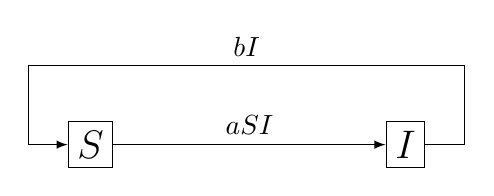
\begin{tikzpicture}
    \node[draw] at (0,0) (S) {\Large $S$};
    \node[draw] at (4,0) (I) {\Large $I$};
    \draw[draw, -latex] (S.east) -- (I.west) node [midway,above] {$aSI$};;
    \draw[draw, -latex] (I.east) -| ($(I.east)+(0.5,1)$) -- ($(S.west)+(-0.5,1)$) node [midway,above] {$bI$} |- (S.west);
    \end{tikzpicture}
    \caption{Diagram of the SIS model}
\end{figure}

$$\frac{dS}{dt} = -aSI + bI$$
$$\frac{dI}{dt} = aSI - bI$$

\subsection{The SEIS model}
As we know, SARS-CoV-2 infection leads an incubation period during which the infected person don't have symptoms but can transmit the infection to other people. We introduce an exposed class $E$ in which we put people that had have a contact with infected people and may be infected in an asymptomatic status.

\paragraph{New classes}
\begin{itemize}
\item $E$ = Exposed
\end{itemize}

\paragraph{New variables}
\begin{itemize}
\item $k$ = probability that exposed people become infective.
\end{itemize}

\begin{figure}
	\centering
    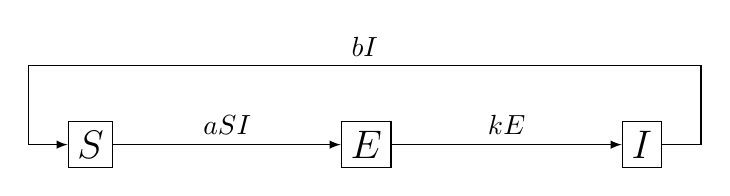
\begin{tikzpicture}
    \node[draw] at (0,0) (S) {\Large $S$};
    \node[draw] at (3.5,0) (E) {\Large $E$};
    \node[draw] at (7,0) (I) {\Large $I$};
    \draw[draw, -latex] (S.east) -- (E.west) node [midway,above] {$aSI$};
    \draw[draw, -latex] (E.east) -- (I.west) node [midway,above] {$kE$};
    \draw[draw, -latex] (I.east) -| ($(I.east)+(0.5,1)$) -- ($(S.west)+(-0.5,1)$) node [midway,above] {$bI$} |- (S.west);
    \end{tikzpicture}
    \caption{Diagram of the SEIS model}
\end{figure}

$$\frac{dS}{dt} = -aSI + bI$$
$$\frac{dE}{dt} = aSI - kE$$
$$\frac{dI}{dt} = kE - bI$$

\paragraph{\textbf{No immunity provided}}
Beacuse of the unknown properties of immunity from SARS-CoV-2, we can assume that the S class and R class coincide, creating a cycle that causes the comeback of the recoverd individuals in the susceptible class.

\subsection{The SEIQJS model}
Due to the unavailability of a vaccine, to fight SARS-CoV-2 infected people are quarantined or isolated (or, also, hospitalized). As suggested from the SEIQJR model, two classes were added: $Q$ is the class of quarantined people, i.e. the exposed people belong to the class $E$; $J$ is the class for isolate infected people of class $I$. So basically $Q$ is for $E$ what $J$ is for $I$, with the only difference that there is a flow from $Q$ to $J$ but not vice versa.\\
People isolated (i.e. belong to class $J$) can recover as people belong to class $I$.

\paragraph{New classes}
\begin{itemize}
\item $Q$ = Quarantined
\item $J$ = Isolated
\end{itemize}

\paragraph{New variables}
\begin{itemize}
\item $\varepsilon_E$ = probability that a person exposed (in $E$) transmit the infection, exposed-transmission-factor;
\item $\varepsilon_Q$ = probability that a person quarantined (in $Q$) make a contact, quarantined-contact-factor;
\item $\varepsilon_J$ = probability that a person isolated (in $J$) transmit the infection, isolation-transmission-factor;
\item $k_E$ = probability that exposed people become infective;
\item $k_Q$ = probability that quarantined people are isolated;
\item $c_Q$ = percentage of exposed people that are quarantined at each time step;
\item $c_J$ = percentage of infected people that are isolated at each time step;
\item $b_I$ = probability that an infected person get recovered;
\item $b_J$ = probability that an isolated person get recovered;
\end{itemize}

\begin{figure}[H]
	\centering
    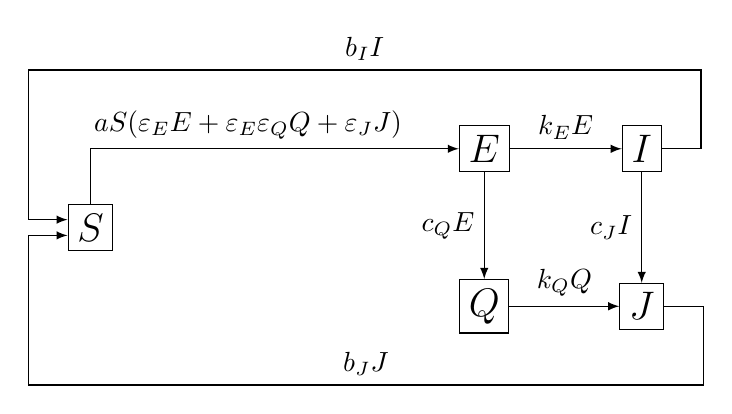
\begin{tikzpicture}
    \node[draw] at (0,0) (S) {\Large $S$};
    \node[draw] at (5,1) (E) {\Large $E$};
    \node[draw] at (5,-1) (Q) {\Large $Q$};
    \node[draw] at (7,1) (I) {\Large $I$};
    \node[draw] at (7,-1) (J) {\Large $J$};
    \draw[draw, -latex] (S.north) |- (E.west) node [midway,xshift=2cm,above] {$aS(\varepsilon_EE + \varepsilon_E\varepsilon_QQ + \varepsilon_JJ)$};
    \draw[draw, -latex] (E.south) -- (Q.north) node [midway,left] {$c_QE$};
    \draw[draw, -latex] (E.east) -- (I.west) node [midway,above] {$k_EE$};
    \draw[draw, -latex] (I.south) -- (J.north) node [midway,left] {$c_JI$};
    \draw[draw, -latex] (Q.east) -- (J.west) node [midway,above] {$k_QQ$};
    \draw[draw, -latex] (I.east) -| ($(I.east)+(0.5,1)$) -- ($(S.west)+(-0.5,2)$) node [midway,above] {$b_II$} |- ($(S.west)+(0,0.1)$);
    \draw[draw, -latex] (J.east) -| ($(J.east)+(0.5,-1)$) -- ($(S.west)-(0.5,2)$) node [midway,above] {$b_JJ$} |- ($(S.west)-(0,0.1)$);
    \end{tikzpicture}
    \caption{Diagram of the SEIQJS model}
\end{figure}

$$\frac{dS}{dt} = -aS(\varepsilon_EE + \varepsilon_E\varepsilon_QQ + \varepsilon_JJ) + b_II + b_JJ$$
$$\frac{dE}{dt} = aS(\varepsilon_EE + \varepsilon_E\varepsilon_QQ + \varepsilon_JJ) - (k_E + c_Q)E$$
$$\frac{dQ}{dt} = c_QE - k_QQ$$
$$\frac{dI}{dt} = k_EE - (b_I + c_J)I$$
$$\frac{dJ}{dt} = k_QQ + c_JI - b_JJ$$

\subsection{Action to limit the epidemic spread}
In a context of epidemic spread some actions can carried on to protect the health of the population. Basically, because of the virus infection is transmitted during contacts person-to-person, these contacts must be reduced. Putting the exposed or infected people in quarantine or isolation is the best thing to do, but also methods of social distancing or mobility restrictions can be used. \\
In this project I implemented quarantine, isolation, social distance and lockdown.

\subsection{Contact tracing and evaluation method}
As we know that SARS-CoV-2 infection leads to an asymptomatic status, a contact tracing technique can be used to find people who can transmit the virus before that they become symptomatic. In this model I built a contact tracing technique not properly to find potential infected individuals, but to evaluate the amount of contacts in each simulation to have an indicator of the power of the spreading. What is important to notice is that the more contacts we have between people, the more powerfull the outbreak will be and thus the harder will be to control it.

\section{Implementation}
In this section I describe the way I implemented the concepts shown in the previous section.

\subsection{The base model}
The Virus model from the NetLogo library \cite{netlogo-virus} is the point from which I started the development of my model. The Virus model is an implementation of the SIR model, with some peculiarities:
\begin{enumerate}
\item people can reproduce;
\item people can recover from the infection but they can also die;
\item recovered individuals have a phase of immunity before they come back to the susceptible class.
\end{enumerate}
I conclude that these three characteristics have no interest to be in my final model, so I edited this model to have the following situation:
\begin{enumerate}
\item people cannot reproduce because the epidemic spread is as fast as we can ignore the machanism of reproduction in the population;
\item people can only recover from the infection and they cannot die;
\item recovered individuals have no phase of immunity beacuse, for SARS-CoV-2, we don't have clear informations.
\end{enumerate}
Once I have a SIR model is easy to transform it to a SIS model: the only thing to do is put the flow that previously went to the recovered class ($R$) in the susceptible class ($S$).\\
After this editing I basically my final model will be an enrichment of this model.

\subsection{Parameters}
The parameters of the model are the ones described for the SEIQJS model, divided into fixed parameters, i.e. the ones that are specific to the virus, and the control parameters, which can be tuned in order to study attempts to manage the epidemic.

\paragraph{Fixed parameters}
\begin{itemize}
\item \texttt{infection-rate} ($a$);
\item \texttt{exposed-transmission-factor} ($\varepsilon_E$);
\item \texttt{exposed-to-infected-rate} ($k_E$);
\item \texttt{quarantined-to-isolated-rate} ($k_Q$);
\item \texttt{infected-chance-recover} ($b_I$);
\item \texttt{isolated-chance-recover} ($b_J$).
\end{itemize}

\paragraph{Control parameters}
\begin{itemize}
\item \texttt{quarantine-perfection-rate} ($\varepsilon_Q$);
\item \texttt{quarantine-perfection-rate} ($\varepsilon_J$);
\item \texttt{quarantines-per-tick-rate} ($c_Q$);
\item \texttt{isolations-per-tick-rate} ($c_J$).
\end{itemize}

Experiments with this model are made by trying different values for control parameters, while fixed parameters remain unchanged.

\subsection{Class representation}
The SIS, SEIS and other similar diagrams have a fundamental constraint: at each time step, a person of the population (i.e. an agent) must belong to one and only one class. This is done by simply add five properities to the agent: one of each indicates a different class, so at each time step, one of these property must be true and the others false.

\subsection{Class transitions methods}
To make possible that a person change class a series of methods were implemented. All of them share a similar structure:
\begin{enumerate}
\item check if the candidate that is going to go to the class actually belongs to a class from which a flow from the two classes is defined (throw an error if not);
\item put to \textit{false} the properties of the person that could hold the value \textit{true};
\item put to \textit{true} the property that indicates the new class.
\end{enumerate}
These methods are \texttt{get-exposed}, \texttt{get-quarantined}, \texttt{get-infected}, \texttt{get-isolated} and \texttt{get-recovered}.

\subsection{Core procedures: setup and go}
Every NetLogo model is based on these two procedures:
\begin{itemize}
\item \texttt{setup} is the function that provides the initialization of the model before every simulation;
\item \texttt{go} is the function that will be executed every time step (tick).
\end{itemize}

\paragraph{The procedure \texttt{setup}} creates the turtles that represent the population and initialize their properties: every turtle is putted in the susceptible class. To create the beginning of virus spreading, after these actions some of the created turtles are picked at random and moved to the exposed class and to the infected class.\\

To understand the explaination of the following procedure \texttt{go} I need to underline first a design choice: I decided to let that some actions occurs more often that others, below I explain which they are an why. To implement this behaviour I used a new variable that counts the days elapsed from the beginning of the simulation, every time \texttt{ticks} is a multiplier of \texttt{ticks-per-days}, days counter advances.\\

\paragraph{The procedure \texttt{go}} calls various other procedures that carried on the simulation and the behaviour of the model, but they are divided into two groups:
\begin{itemize}
\item \textit{once-per-tick} procedures that are called every time the \texttt{go} procedure is called, so every tick
\begin{itemize}
\item people motion in the enviroment, 
\item people transition to exposed class due to a contact with an infected person,
\item contract tracing update;
\end{itemize}
\item \textit{once-per-day} procedures that are called every time the days counter advanced:
\begin{itemize}
\item every class transition except the one from susceptible to exposed, that, as I said previously, happens for every tick.
\end{itemize}
\end{itemize}

\subsection{Virus propagation}
The infection spreading of the virus in the population is implemented in the function \texttt{infect} that looks a little bit complicated but, essentialy, uses the parameters of the model call, in a proper way, the procedure \texttt{get\_exposed}. It's the only procedure that makes call to \texttt{get\_exposed}. Take a look to the comments in the code of the model to know more.

\subsection{Contact tracing}
Contact tracing is implemented using the construct \texttt{link} of NetLogo. Ar each time step, the program asks to each person to create a link with other people that share, in that moment, the same patch. Basically is the same way that the virus spreads and it has a sense beacuse the aim of contact tracing is to track the propagation of the virus. The result is a graph connecting people to each others.

\subsection{Social distance and lockdown}
Two methods were implemented to control people movement in order to reduce contacts between them: social distance and lockdown
\paragraph{Social distance} can be enabled or disabled in this model and uses an auxiliry parameter called \texttt{social-distance-perfection-rate}. If social distance is disabled, people are free to move everywhere, while if it's enabled people avoid to move to a patch that is already occupied by others with an error probability of determined by $1 - \textrm{\texttt{social-distance-perfection-rate}}$.
\paragraph{Lockdown} is implemented taking into account a value that defines the probability that a person will move or not. If the variable \texttt{lockdown-strinctness} is set to zero, people are completely free to move, while if the value increases, people will make a move with less probability. If a person doesn't move, it remain in the same patch where it was previously.\\ \\
Take a look to the procedure \texttt{move} to find the code about these control measures.


\subsection{Evaluation}
In this model I consider to evaluate every situation analyzing the graph generate by the contact tracing method. The more connected is the graph, the more powerful is the virus spreading and so, in a real situation, the more stressed the health system will be.\\
I use the definition of \textit{degree centrality} to have a clear indicator of the connections that each person create during simulation. Beacause of degree centrality is a node-based measure, I used the average of all the degree centrality to get a value to evaluate the entire graph. An auxiliary indicator of standard deviation for this average is provided. \\
If a control action on the population reduces the value of \textit{average degree centrality}, it means that the action is effective.

\section{Results}\label{results}
In this section I describe the results obtained with simulations on this model. Differences between simulations are about managing control parameters in order to watch how the simulation evolves with different actions.\\
The size of the population at the beginning of the simulation is fixed at 150 and the duration of the simulation is 365 days.

\subsection{Virus diffusion without actions}

\begin{figure}[H]
	\centering
	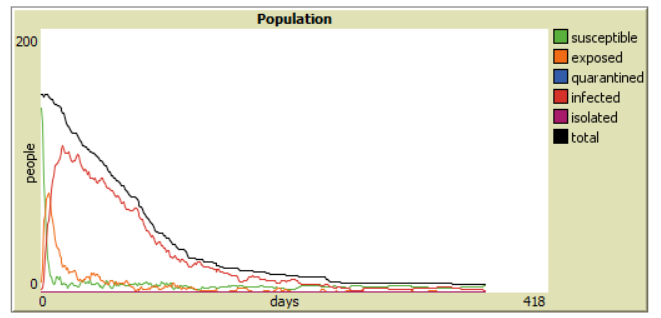
\includegraphics[width=\textwidth]{results/no_actions_population.png}
	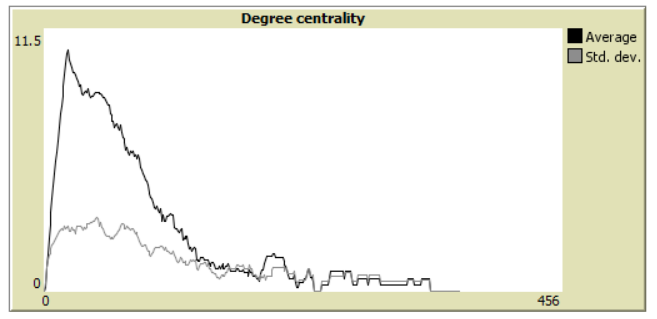
\includegraphics[width=\textwidth]{results/no_actions_degree_centrality.png}
	\caption{Result of the simulations without actions to control the diffusion of the virus. Population has been reduced by \textbf{96\%} and \textbf{147} people were dead.}
\end{figure}

\subsection{Using only quarantine and isolation}
Simulation is carried out with these settings:
\begin{itemize}
\item \texttt{quarantine-perfection-rate} = 70
\item \texttt{quarantines-per-day-rate} = 10
\item \texttt{isolation-perfection-rate} = 90
\item \texttt{isolations-per-day-rate} = 10
\end{itemize}

\begin{figure}[H]
	\centering
	\begin{tikzpicture}
	\node[inner sep=0pt] at (0,0) {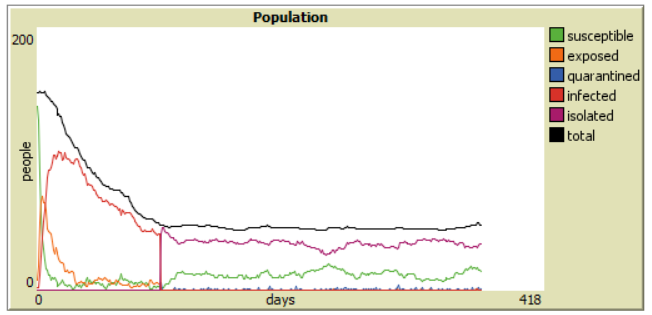
\includegraphics[width=\textwidth]{results/quarantine_isolation_population.png}};
	\node[text width=4cm,align=left] (label) at (0,1) {Activation of quarantine and isolation};
	\draw [->] (label.west) -| (-3.1,-1);
    \end{tikzpicture}
    \begin{tikzpicture}
	\node[inner sep=0pt] at (0,0) {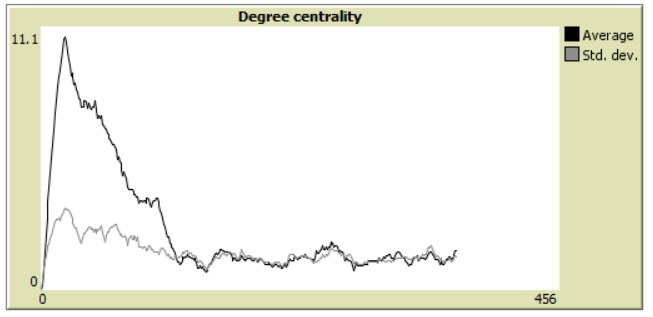
\includegraphics[width=\textwidth]{results/quarantine_isolation_degree_centrality.png}};
	\node[text width=4cm,align=left] (label) at (0,1) {Activation of quarantine and isolation};
	\draw [->] (label.west) -| (-3.2,-0.50);
    \end{tikzpicture}
	\caption{Result of the simulations where on the 100\textsuperscript{th} day quarantine and isolation has been activated for exposed and infected. Population has been reduced by \textbf{66.7\%} and \textbf{122} people were dead.}
\end{figure}

\subsection{Using only social distance and lockdown}
Simulation is carried out with these settings:
\begin{itemize}
\item \texttt{social-distance-perfection-rate} = 70
\item \texttt{lockdown-strictness} = 90
\end{itemize}

\begin{figure}[H]
	\centering
	\begin{tikzpicture}
	\node[inner sep=0pt] at (0,0) {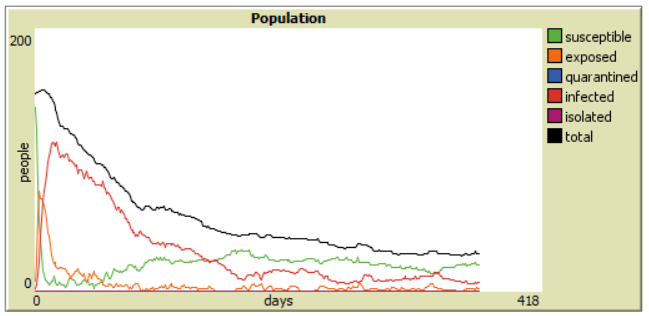
\includegraphics[width=\textwidth]{results/social_distance_lockdown_population.png}};
	\node[text width=2.5cm,align=left] (labela) at (0,1) {Activation of social distance};
	\node[text width=2.5cm,align=left] (labelb) at (0,0) {Activation of lockdown};
	\draw [->] (labela.west) -| (-4.3,0.2);
	\draw [->] (labelb.west) -| (-3.3,-0.8);
    \end{tikzpicture}
    \begin{tikzpicture}
	\node[inner sep=0pt] at (0,0) {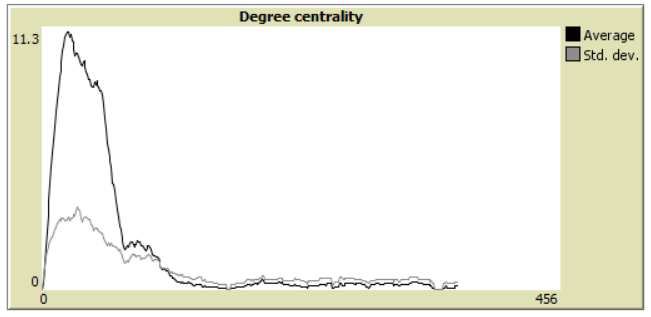
\includegraphics[width=\textwidth]{results/social_distance_lockdown_degree_centrality.png}};
	\node[text width=2.5cm,align=left] (labela) at (0,1) {Activation of social distance};
	\node[text width=2.5cm,align=left] (labelb) at (0,0) {Activation of lockdown};
	\draw [->] (labela.north) -- (0, 2) -| (-4.3,1.6);
	\draw [->] (labelb.west) -| (-3.2,-1.5);
    \end{tikzpicture}
	\caption{Result of the simulations where on the 50\textsuperscript{th} day social distance has been activated for exposed and infected and on the 100\textsuperscript{th} day lockdown has been activated. Population has been reduced by \textbf{80.7\%} and \textbf{163} people were dead.}
\end{figure}

\subsection{Combining quarantine and isolation with social distance and lockdown}

\begin{figure}[H]
	\centering
	\begin{tikzpicture}
	\node[inner sep=0pt] at (0,0) {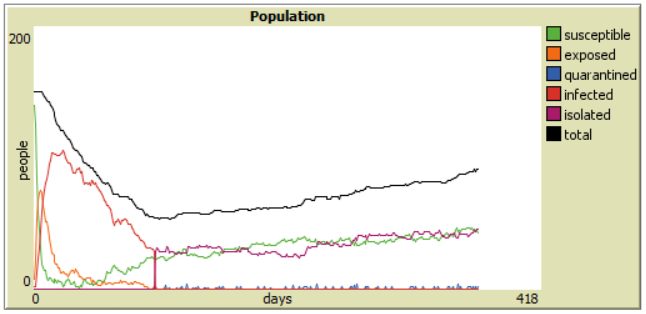
\includegraphics[width=\textwidth]{results/all_methods_population.png}};
	\node[text width=2.5cm,align=left] (labela) at (0,2) {Activation of social distance};
	\node[text width=3.5cm,align=left] (labelb) at (0,1) {Activation of quarantine and isolation};
	\node[text width=2.5cm,align=left] (labelc) at (0,0) {Activation of lockdown};
	\draw [->] (labela.west) -| (-4.3,0.2);
	\draw [->] (labelb.west) -| (-3.2,-0.8);
	\draw [->] (labelc.west) -| (-2.1,-0.8);
    \end{tikzpicture}
    \begin{tikzpicture}
	\node[inner sep=0pt] at (0,0) {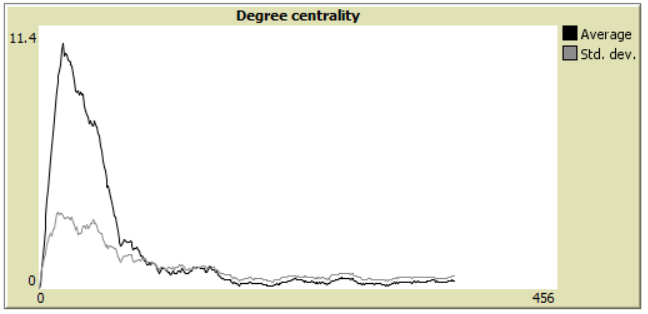
\includegraphics[width=\textwidth]{results/all_methods_degree_centrality.png}};
	\node[text width=2.5cm,align=left] (labela) at (0,1) {Activation of social distance};
	\node[text width=3.5cm,align=left] (labelb) at (0,0) {Activation of quarantine and isolation};
	\node[text width=3.5cm,align=left] (labelc) at (0,-1) {Activation of lockdown};
	\draw [->] (labela.north) -- (0, 2) -| (-4.3,0.8);
	\draw [->] (labelb.west) -| (-3.2,-1.8);
	\draw [->] (labelc.west) -| (-2.1,-1.9);
    \end{tikzpicture}
	\caption{Result of the simulations where on the 50\textsuperscript{th} day social distance has been activated, on the 100\textsuperscript{th} day quarantine and isolations for exposed and infected has been activated and on the 150\textsuperscript{th} day lockdown has been activated. Population has been reduced by \textbf{39.3\%} and \textbf{116} people were dead.}
\end{figure}

\section{Conclusions}\label{conclusions}
We worked hard, and achieved very little.

\printbibliography[title={References}]

\end{document}